\documentclass[a4paper,11pt]{article}
\usepackage{fullpage}
\usepackage{standalone}
\usepackage[utf8]{inputenc}
\usepackage[british]{babel}
\usepackage{csquotes}
\usepackage[T1]{fontenc}
\usepackage{amsmath}
\usepackage{amssymb}
\usepackage{mathtools}
\usepackage{mathptmx}
\usepackage{natbib}
\usepackage[final,babel]{microtype}
\usepackage[colorlinks,linkcolor=blue,citecolor=blue,urlcolor=blue]{hyperref}
\usepackage{doi}
\usepackage{siunitx}
\usepackage[margin=3pt]{subcaption}
\usepackage{xcolor}
\PassOptionsToPackage{final}{graphicx}
\usepackage{tikz}
\usetikzlibrary{arrows}
\usetikzlibrary{patterns}
\usepackage{bm}
\usepackage{booktabs}
\usepackage{tabularx}
\usepackage{enumitem}
\usepackage{titlesec}

\title{
\vspace*{-2em}
Monitoring Committee Progress Report \#5\\
\vspace*{1em}
\Large{Numerical Representation of Mountains in Atmospheric Models}}
\author{James Shaw
\vspace{0.5em} \\
\large{Supervisors: Hilary Weller, John Methven, Terry Davies}
\vspace{0.5em} \\
\large{Monitoring Committee: Paul Williams, Maarten Ambaum}}
\date{June 2017}

\captionsetup{margin=3pt,font={small}}
\setlength{\bibsep}{0.3em plus 0.1ex}

\makeatletter
\AtBeginDocument{
  \hypersetup{
    pdftitle = {Monitoring Committee Progress Report \#5},
    pdfauthor = {James Shaw}
  }
}
\makeatother

\makeatletter
\patchcmd{\ttlh@hang}{\parindent\z@}{\parindent\z@\leavevmode}{}{}
\patchcmd{\ttlh@hang}{\noindent}{}{}{}
\makeatother

\newcommand{\iu}{{i\mkern1mu}}
\newcommand{\TODO}[1]{\textcolor{purple}{TODO: \emph{#1}}}

\defcitealias{openfoam}{{OpenFOAM user guide}}
\begin{document}
\maketitle

\section{Introduction}

Numerical weather forecast and climate prediction models are using increasingly fine horizontal meshes to resolve small-scale features and make forecasts more accurate.  Traditionally, atmospheric models have used uniform latitude-longitude meshes to represent a spherical Earth with terrain-following vertical coordinates to represent Earth's terrain, but these representations become problematic with fine horizontal mesh spacing.
First, the cells of latitude-longitude meshes are very small near the Earth's poles, causing a bottleneck in parallel computation \citep{staniforth-thuburn2012} and placing severe time-step constraints on explicit Eulerian methods.
Second, computer storage and computation time increase dramatically when horizontal mesh spacing is reduced uniformly over a latitude-longitude mesh: halving the horizontal mesh spacing results in four times as many cells and simulations require a smaller time-step.
Third, fine horizontal meshes resolve small-scale steep slopes that severely distort terrain-following coordinate surfaces, resulting in larger numerical errors \citep{schaer2002} or even numerical instability \citep{webster2003}.

In response to these problems, a variety of alternative horizontal and vertical representations have been proposed.  Alternative, quasi-uniform meshes avoid small cells near the poles of latitude-longitude meshes \citep{staniforth-thuburn2012}.  Some models are already using quasi-uniform meshes: the German ICON model uses an icosahedral mesh \citep{wan2013}, the Canadian GEM model uses a yin-yang mesh comprising two overlapping sections arranged like a tennis ball \citep{qaddouri2011}, and the UK Met Office are preferring a cubed-sphere mesh for their next-generation Gung-Ho model (Nigel Wood 2017, personal communication).
To improve the scalability of computational resources with finer mesh spacing, static mesh refinement and dynamic adaptive mesh techniques create meshes with fewer cells while retaining the numerical accuracy achieved with a uniformly fine mesh \citep{jablonowski2009}.
mprovements have also been made to the vertical representation over steep terrain.  Mesh distortions are less severe when terrain-following coordinates are smoothed \citep{leuenberger2010,klemp2011}, and cut cell meshes are orthogonal everywhere except at the ground.

These alternative meshes alleviate many of the computational and numerical problems that arise due to finer horizontal mesh spacing, but they introduce problems of their own.
Unlike latitude-longitude meshes, quasi-uniform meshes have non-zero skewness or non-orthogonality that produces grid imprinting errors and excites computational modes \citep{weller2012}.
Mesh refinement and adaptive mesh techniques also create mesh geometries with non-orthogonalities or hanging nodes \citep{marras2016}.
Cut cell meshes are orthogonal nearly everywhere but the cut cell method creates arbitrarily small cells that impose severe time-step constraints on explicit Eulerian methods \citep{klein2009}.

This PhD makes three contributions to improve numerical accuracy on arbitrary meshes.  First, a new mesh for representing steep terrain avoids the severe distortions associated with terrain-following meshes \citep{shaw-weller2016} and avoids severe time-step constraints associated with cut cell meshes \citep{shaw2017}.  Second, a new advection scheme is formulated for numerical stability on high-distorted meshes \citep{shaw2017}.  It is second-order convergent on quasi-uniform spherical meshes, terrain-following and cut cell meshes.
Third, the Charney--Phillips staggering of variables is generalised for arbitrary meshes and is shown to eliminate the computational mode associated with a Lorenz staggering.

The OpenFOAM computational fluid dynamics library is used throughout the project to enable like-for-like comparisons.  Different types of mesh are compared using the same model, and different variable staggerings are compared using variants of a single model.
The PhD also contributes two new two-dimensional test cases that are suitable for evaluating dynamical cores.  The first test challenges advection schemes near steeply-sloping lower boundaries \citep{shaw2017}.
The second test is designed to excite the Lorenz computational mode.  Existing tests that excite the Lorenz computational mode are poorly suited to dynamical core evaluation: the standing waves test by \citet{arakawa-konor1996} was designed for a model with no horizontal discretisation, and the radiative heating test by \cite{untch-hortal2004} requires a 600-day integration using a three-dimensional spherical Earth.  The test that we propose requires a 2-day integration using a two-dimensional Cartesian plane and is based on the test by \citet{arakawa-konor1996}.


\section{Advection over steep slopes on arbitrary meshes}
We submitted a manuscript to the Journal of Computational Physics in February 2017 documenting the finite volume advection scheme, ``cubicFit''.  The final article \citep{shaw2017} was made available in April 2017 after one round of minor corrections.  The cubicFit scheme is largely insensitive to mesh distortions and maintains second-order convergence on highly distorted meshes.  Idealised tests demonstrate that the cubicFit scheme is more stable and more accurate than a standard multidimensional linear upwind scheme.

Having presented our work at PDEs on the Sphere in April \href{http://crd.lbl.gov/departments/applied-mathematics/ANAG/about/staff-and-postdocs/hans-johansen/}{Hans Johansen}, a researcher from the computational research group at Lawrence Berkley National Lab, told me that his group have developed a high-order finite volume scheme for solving Poisson's equation on cut cell meshes \citep{devendran2015}.  Hans is keen to help me apply these techniques to the cubicFit advection scheme in order to achieve convergence higher than second-order.  If time permits, I hope to collaborate with Hans to take this work further.

\section{Generalisation of Charney--Phillips for arbitrary meshes}

The Charney--Phillips vertical staggering of variables \citep{charney-phillips1953} is suitable for structured meshes with cells stacked in columns. This staggering has been adopted by several operational models \citep{davies2005,yang2007,girard2014} because it avoids the computational mode that is associated with the Lorenz vertical staggering \citep{arakawa-konor1996}. The generalisation of the Lorenz staggering for unstructured or arbitrarily-structured meshes is straightforward \citep{weller-shahrokhi2014} but this is not true for the Charney--Phillips staggering.

On a finite volume mesh, variables are ordinarily placed at cell centres or cell faces. In the Charney--Phillips staggering, the thermodynamic variable is placed at only those cell faces that lie on vertical coordinate surfaces, and vertically-oriented faces have no thermodynamic information. This arrangement is unsuitable for arbitrarily-structured finite volume meshes because faces can have any orientation.

\begin{figure}
\centering
\documentclass[tikz]{standalone}
\usepackage{times}
\usepackage{bm}
\begin{document}
\begin{tikzpicture}[
  scale=0.5,
  cpnt/.style={fill=gray}
]

\draw (2,3) -- (0,7) -- (7,9) -- (7,0) -- (2,3);

\path [cpnt] (4.1,5) circle [radius=0.2] node [right] {$\theta_C$};

\draw [thick] (7,4.5) circle [radius=0.2];
\draw [thick] (4.5,1.5) circle [radius=0.2];
\draw [thick] (3.5,8) circle [radius=0.2];
\draw [thick] (1,5) circle [radius=0.2];

\end{tikzpicture}
\end{document}

	\caption{A quadrilateral cell with the prognostic thermodynamic variable $b_f$ stored at face centres marked by open circles.  $b_f$ is calculated from the potential temperature $\theta_f$ such that $b_f = \theta_f \mathbf{\hat{g}} \cdot \mathbf{\hat{n}}_f$ where $\mathbf{\hat{n}}_f$ is the unit vector outward normal to face $f$, and $\mathbf{\hat{g}}$ is the unit vector of gravitational acceleration.  The potential temperature at the cell centre, $\theta_C$, is reconstructed from surrounding values of $b_f$ using equation~\eqref{eqn:reconstruct}.}
\label{fig:cp-staggering}
\end{figure}

Work is on schedule to develop a generalisation of the Charney--Phillips staggering of variables.  The prognostic thermodynamic variable $b_f$ is stored at all cell faces such that $b_f = \theta_f \mathbf{\hat{g}} \cdot \mathbf{\hat{n}}_f$ where $f$ is a face, $\theta_f$ is the potential temperature, $\mathbf{\hat{g}}$ is the unit vector of gravitational acceleration and $\mathbf{\hat{n}}_f$ is the unit vector that is outward normal to the face.
This arrangement is illustrated in figure~\ref{fig:cp-staggering}.

To outline the discretisation, let us consider its application to a Cartesian mesh with no diagonal faces.  First, potential temperature is transported in advective form,
\begin{align}
	\theta_f^{n+1} = \theta_f^{\ell} - \Delta t \mathbf{U}_f \cdot \left( \nabla_c \theta_f \right)_F
\end{align}
where $\theta_f^{n+1}$ is the value of $\theta_f$ at the new time-step, $\theta_f^\ell$ is the lagged value from the previous solver iteration, $\mathbf{U}_f$ is the wind, $\left( \cdot \right)_F$ denotes an interpolation from cell centres to faces, and $\nabla_c$ denotes a cell centre gradient \citep{weller-shahrokhi2014}.
Next, $b_f$ is calculated such that $b_f = \theta_f \mathbf{\hat{g}} \cdot \mathbf{\hat{n}}_f$.  
On a Cartesian mesh, $b_f$ is zero for entirely vertical faces and $b_f = \theta_f$ for entirely horizontal faces.

Where potential temperature is required at the cell centre, it is reconstructed from bordering faces,
\begin{align}
	\theta_C &= \mathbf{\hat{g}} \cdot \left( \sum_{f \in c} \mathbf{\hat{n}}_f \mathbf{S}_f \right)^{-1} \cdot \sum_{f \in c} \mathbf{S}_f b_f \label{eqn:reconstruct}
\end{align}
where $\theta_C$ is the reconstructed potential temperature, $f \in c$ denotes the faces $f$ bordering cell $c$, and $\mathbf{S}_f$ is the vector with magnitude equal to the face area and an outward normal direction.  On a Cartesian mesh, $\theta_C$ is simply a linear interpolation from the face values immediately above and below the cell centre.

Finally, $\theta_f$ is recalculated from $b_f$ and $\theta_C$,
\begin{align}
	\theta_f = \lvert \mathbf{\hat{g}} \cdot \mathbf{\hat{n}}_f \theta_f \rvert + \left( 1 - \lvert \mathbf{\hat{g}} \cdot \mathbf{\hat{n}} \rvert \right) \left( \theta_C \right)_F \text{.}
\end{align}
This ensures that values of $\theta_f$ on vertical faces is calculated from nearby $b_f$ values and is not retained across time-steps.
We have created a new variant of the nonhydrostatic model by \citet{weller-shahrokhi2014} that implements this generalised Charney--Phillips formulation.

We have also created a new two-dimensional vertical slice test case that we use to compare the Lorenz and generalised Charney--Phillips model variants.
The new test case is based on the standing waves test by \citet{arakawa-konor1996}, which was designed for a vertically discrete model with no horizontal discretisation.
Grid-scale potential temperature perturbations are added to an isothermal atmosphere in hydrostatic balance (figure~\ref{fig:waves-initial}).  The details of the test configuration have yet to be finalised.

After a two day integration, preliminary results using the Lorenz model show a spurious grid-scale oscillation occupying the entire depth of the domain, having propagated upwards from the position of the initial perturbation (figure~\ref{fig:waves-lorenz}).  This grid-scale error indicates that the Lorenz computational mode has been excited.  No such error is found with the generalised Charney--Phillips model (figure~\ref{fig:waves-cp}).

\begin{figure}
\centering
\subcaptionbox{Initial potential temperature perturbation \label{fig:waves-initial}}[.32\linewidth]{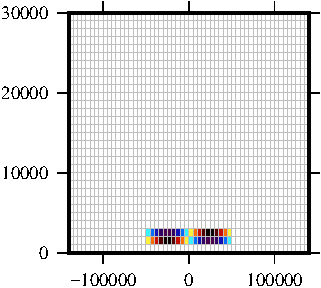
\includegraphics{initial-theta-diff.pdf}}
\subcaptionbox{Final result using the Lorenz model \label{fig:waves-lorenz}}[.32\linewidth]{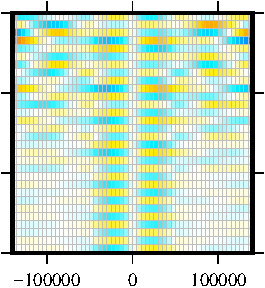
\includegraphics{lorenz-theta-diff.pdf}}
\subcaptionbox{Final result using the generalised Charney--Phillips model \label{fig:waves-cp}}[.32\linewidth]{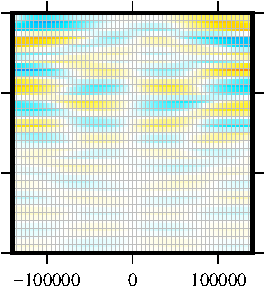
\includegraphics{cp-theta-diff.pdf}}
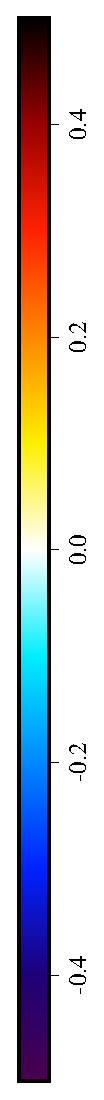
\includegraphics[height=5.5in,angle=270]{theta-diff-legend.eps}
\caption{Potential temperature perturbations from the isothermal state in the two-dimensional standing waves test case.  Initially, grid-scale perturbations with a maximum amplitude of $\pm \SI{0.5}{\kelvin}$ are added in the centre of the domain near the ground.  These perturbations generate gravity waves that spread through the domain.  A spurious grid-scale oscillation indicates that the Lorenz computational mode is excited using the Lorenz model.  No such error is present using the generalised Charney--Phillips model.
Only the central part of the domain is shown with cell edges marked by grey lines.
Axes are in units of metres.
}
\label{fig:cp-results}
\end{figure}

\section{Future research}

%Work is on track according to the schedule set out in MC4.

\subsection*{A third paper?}
\TODO{
Do we want to get another paper out before submitting?  If so, what is a minimum viable paper?
\begin{itemize}
	\item A generalised formulation of Charney--Phillips for arbitrary meshes
	\item A Charney--Phillips OpenFOAM model with reasonably accurate non-orthogonal treatment
	\item The new standing waves test case with a comparison of results:
	\begin{itemize}
		\item uniform mesh, meshes with non-conformal block refinement and conformal refinement (with diagonal faces)
		\item Lorenz and Charney--Phillips model variants to demonstrate the presence and absence of the Lorenz computational mode respectively
	\end{itemize}
\end{itemize}
Additionally and, in my opinion, optionally, the paper could include
\begin{itemize}
	\item Try the standing waves test over orography
	\item Improved $\theta$ advection in Charney--Phillips model, possibly similar to cubicFit in advective form
	\item Evaluate the $\theta$ advection scheme using a variant of the \citet{schaer2002} gravity waves test that incorporates standing waves that excite the Lorenz computational mode
\end{itemize}
}

\subsection*{Timeline of work}

\TODO{
Do I need to discuss a possible extension of funding at this meeting?  If so:
\begin{itemize}
	\item I've spent a lot of time writing papers, including a total of five months revising manuscripts (details in Appendix C)
	\item I've also taken two Masters modules, one of which was assessed
	\item Do I want to budget some time for making the cubicFit scheme high-order?
	\item Does 1 month per chapter sound reasonable?  If so, I could likely be finished by January, but only if I don't write a third paper.
\end{itemize}
}


% June
%  - improve CP model
% July
%  - high-order cubicFit
% August
%  - complete cubicFit chapter
% September
%  - complete slanted cell chapter
% October
%  - complete C--P chapter
% November
%  - complete existing methods chapter
% December
%  - complete introduction



\section{Personal development}

Since the last monitoring committee meeting in November 2016 I have been invited to speak at the RMetS south-east meeting at the University of Reading, and at a numerical methods workshop at Imperial College.  I am helping to organise the NERC student conference, lead by students from NERC DTPs in London, and I have applied to present at SciCADE, a conference on scientific computation and differential equations.

I am now considering my options for future employment, and I am keen to continue research in numerical methods, either applied to weather and climate modelling or other disciplines.
Hilary has kindly introduced me to a number of colleagues in UK institutions and I am following up with those who may have positions opening soon.

I am also interested other academic roles that promote good practices in reproducible science and research software engineering.
I have applied for a 10-month Mozilla science fellowship that supports researchers wanting to promote open science within their institution.
The international programme selects four fellows each year, with this year's fellows being chosen in June 2017.
Mozilla allow fellows to spend 20\% of their time on their own research and so, should I be chosen, I would need to work on my PhD part-time and postpone the completion date for 8 months.

If I cannot find a suitable academic job I am considering computational fluid dynamics positions and software engineering positions elsewhere.
I submitted an application in May to the UK Met Office who have several software engineering vacancies.


\bibliographystyle{ametsoc2014}                                                 
\bibliography{references}

\newpage

\titlespacing\subsubsection{0pt}{0.8em plus 4pt minus 2pt}{0.2em plus 2pt minus 2pt}

\section*{Appendix A: Thesis plan}
The thesis chapters are expected to be as follows:

\subsubsection*{Introduction}
\noindent This project is motivated by the need for alternative horizontal and vertical representations of the Earth and its terrain.

\subsubsection*{Existing methodologies}
\begin{itemize}[itemsep=0.1em]
	\item Describe Lorenz and Charney--Phillips staggerings for structured quadrilateral meshes
	\item Describe the nonhydrostatic finite volume model with Lorenz staggering for arbitrary meshes \citep{weller-shahrokhi2014}
\end{itemize}

\subsubsection*{A new mesh for representing terrain}
\noindent The slanted cell mesh improves pressure gradient accuracy and avoids severe timestep constraints for explicit methods.
\begin{itemize}[itemsep=0.1em]
	\item Introduce existing types of mesh: terrain-following layers and cut cells
	\item Describe the new slanted cell method
	\item A two-dimensional test of a quiescent atmosphere above steep slopes, comparing terrain-following, cut cell and slanted cell meshes (using the linearUpwind scheme?)
\end{itemize}

\subsubsection*{A new transport scheme for steep slopes}
\noindent The cubicFit transport scheme is stable and accurate over steep slopes with arbitrary, distorted meshes.
\begin{itemize}[itemsep=0.1em]
	\item Document the cubicFit transport scheme
	\item {Test results comparing linearUpwind and cubicFit transport schemes
	\begin{itemize}[itemsep=0.1em,topsep=0pt]
		\item \citet{shaw2017} transport test over steep slopes 
		\item \citet{lauritzen2012} deformational transport tests on a spherical Earth
		\item \citet{schaer2002} mountain waves test case (should demonstrate that cubicFit is necessary to obtain the reference solution)
	\end{itemize}}
\end{itemize}

\subsubsection*{Possible extension: making the cubicFit transport scheme high-order}
\noindent Hans Johansen is keen to help me improve the cubicFit scheme.  I should start with advection on non-uniform, one-dimensional meshes before attempting advection in the interior of arbitrary, two-dimensional meshes.  I do not expect to investigate discretisation issues near domain boundaries.
	
\subsubsection*{A generalisation of the Charney--Phillips staggering}
\noindent The Charney--Phillips staggering avoids the Lorenz computational mode, but it has only been formulated for structured quadrilateral meshes.  A generalised formulation will be suitable for arbitrary meshes, including the slanted cell mesh.
\begin{itemize}[itemsep=0.1em]
	\item Describe the generalised Charney--Phillips formulation
	\item Describe the necessary changes to the nonhydrostatic model of \citet{weller-shahrokhi2014}
	\item Compare results between the Lorenz and Charney--Phillips variants of the model using the two-dimensional standing waves test case
\end{itemize}

\subsubsection*{Possible extension: grid-scale perturbations over orography}
\noindent We should demonstrate the efficacy of combining all three work items: the slanted cell mesh, the cubicFit transport scheme, and the generalised Charney--Phillips formulation.  In order to achieve this, we may be able to incorporate the grid-scale perturbations from the standing waves test into the mountain waves test case by \citet{schaer2002}.
Results should be compared between Lorenz and Charney--Phillips model variants and between mesh types.

\newpage

\section*{Appendix B: Training record}

\subsubsection*{Mathematics modules}
\footnotesize
\begin{tabular}{l l l l}
Spring 2017	& \href{https://finite-element.github.io}{M5A47}  & Finite elements: numerical analysis and implementation & unassessed, partially completed \\
Spring 2016	& \href{www.reading.ac.uk/module/document.aspx?modP=MA3NAT&modYR=1516}{MA3NAT} & Numerical Analysis II & unassessed \\
Spring 2015	& \href{www.reading.ac.uk/modules/document.aspx?modP=MAMNSP&modYR=1415}{MAMNSP} & Numerical Solution of Partial Differential Equations  & 78\% \\
\end{tabular}

\subsubsection*{RRDP modules}
\begin{tabular}{l l}
23 June 2017    & Graduate school conference \\
3 May 2017	& Effective CVs \\
28 Feb 2017	& Getting your first post-doc position \\
9 Nov 2016      & Open Access and research data management \\
24 Mar 2016	& Voice coaching: looking after your voice \\
26--27 Jan 2016 & Preparing to teach (introduction, marking \& feedback, leading small groups) \\
2 Dec 2015	& An essential guide to critical academic writing \\
17 Nov 2015	& Understanding the UK higher education context \\
19 May 2015	& How to avoid plagiarism \\
10 Mar 2015	& How to write a literature review \\
19 Feb 2015	& How to write a paper \\
\end{tabular}

\subsubsection*{External courses}
\begin{tabular}{l l}
June 2016 & Dynamical core intercomparison project summer school, NCAR \\
13 May 2016 & Peer review: the nuts and bolts, Sense about Science \\
June 2015 & Advanced numerical methods for Earth-system modelling, ECMWF \\
\end{tabular}

\subsubsection*{Conferences and workshops}
\begin{tabularx}{\linewidth}{l l X}
September 2017 & Applicant & \href{https://sites.google.com/site/scicade2017/}{International conference on scientific computation and differential equations}, University of Bath \\
August 2017 & Co-organiser & NERC student conference (working title) \\
July 2017 & Speaker & UK Met Office GungHo network meeting, University of Exeter \\
June 2017 & Participant & \href{https://www.software.ac.uk/c4rr}{Docker containers for reproducible research}, University of Cambridge \\
April 2017 & Speaker & \href{https://forge.ipsl.jussieu.fr/heat/wiki/PDEs2017}{PDEs on the Sphere}, École normale supérieure, Paris \\
March 2017 & Attendee & \href{https://blogs.reading.ac.uk/open-research/open-in-practice-inspirations-strategies-and-methods-for-open-research/}{Open in practice: inspirations, strategies and methods for open research}, University of Reading \\
March 2017 & Participant & \href{http://www.effective-quadratures.org/eq2017}{Effective quadratures workshop}, University of Cambridge \\
February 2017 & Invited speaker & Numerical methods for geophysical fluid dynamics, Imperial College London \\
January 2017 & Attendee & Research software management, sharing and sustainability, British Library \\
December 2016 & Invited speaker & \href{https://www.rmets.org/events/meteorological-research-within-university-reading-2016}{South-East local centre meeting, Royal Meteorological Society} \\
October 2016 & Speaker & \href{http://www.ecmwf.int/en/learning/workshops-and-seminars/workshop-numerical-and-computational-methods-simulation-all-scale-geophysical-flows}{Numerical and computational methods for simulation of all-scale geophysical flows}, ECMWF \\
November 2015 & Attendee & GungHo workshop on next generation weather and climate prediction, UK Met Office \\
June 2015 & Attendee & Hoskins@70 \\
June 2015 & Poster & SCENARIO DTP conference \\
March 2015 & Speaker & \href{http://www.icms.org.uk/workshop.php?id=334}{Galerkin methods with applications in weather and climate forecasting}, ICMS \\
\end{tabularx}

\subsubsection*{Teaching}
\begin{tabular}{l l l}
Oct 2016 & Teaching assistant & MTMW11 fluid dynamics \\
Oct 2015 & Teaching assistant & MTMG02 atmospheric physics \\
Sep 2015 & Teaching assistant & NCAS summer school \\
Sep 2014 & Course teacher & MPE python and linux short course \\
\end{tabular}

\subsubsection*{Visits and collaborations}
\begin{tabularx}{\linewidth}{l X}
July 2016 & Organised visit from \href{https://www.youtube.com/user/SimonOxfPhys}{Simon Clark}, stratospheric PhD researcher and YouTube vlogger \\
Summer 2016 & Worked with Hilary's MSc student, Christiana Skea, studying variable timestepping for ODEs \\
June 2016 & Visited NCAR, hosted by Ram Nair \\
2015 -- 2017 & Coauthoring an article about dimensionally-split and multidimensional transport schemes, written with Hilary, her former student \href{https://www.clisap.de/research/a:-climate-dynamics-and-variability/crg-numerical-methods-in-geosciences/team-members/yumeng-chen/}{Yumeng Chen}, and Stephen Pring at the UK Met Office \\
\end{tabularx}

\subsubsection*{Outreach}
\begin{tabular}{l l l}
17 Mar 2017 & ``\href{https://thesocialmetwork.wordpress.com/2017/03/17/simulating-wind-on-computers/}{The advection process: simulating wind on computers}'', Social Metwork blog article \\
14 Jul 2015 & Schools physicist of the year awards \\
14 Jun 2015 & East Reading festival \\
15 Feb 2015 & Brighton science festival \\
\end{tabular}

\subsubsection*{Presentations}
\begin{tabularx}{\linewidth}{l l X}
19 Jun 2017 & HHH group & Quantifying uncertainty with effective sub-sampling (working title) \\
30 Mar 2017 & Mesoscale group & Modern advection schemes for weather and climate models (working title) \\
17 Nov 2016 & Comp. Atmos. Dyn. group & A review of atmospheric transport schemes \\
9 Nov 2016 & PhD group & Replicable computational atmospheric science \\
31 Oct 2016 & HHH group & Advection over steep slopes \\
22 Sep 2016 & PhD poster session & Improving numerical accuracy over steep slopes \\
23 Mar 2016 & Quo Vadis & Numerical representation of orography in dynamical cores (honourable mention) \\
17 Feb 2016 & PhD group & Multidimensional advection schemes for arbitrary meshes \\
9 Feb 2016 & Mesoscale group & Curl-free pressure gradients for accurate modelling of cold air pools \\
19 Oct 2015 & HHH group & Improving modelled mountain flows with alternative representations of terrain \\
27 Apr 2015 & HHH group & A like-for-like comparison between terrain following and cut cell grids \\
21 Apr 2015 & PhD group & Discrete vector calculus on Arakawa C grids \\
12 Feb 2015 & UK Met Office & Poster presentation for Met Office Academic Partnership \\
18 Jan 2015 & PhD group & Python and linux tips \\
17 Dec 2014 & MPECDT jamboree & Poster presentation for Mathematics for Planet Earth Centre for Doctoral Training jamboree \\
12 Sep 2014 & Lunchtime seminar  & Gain control of your documents and code: hands-on with revision control and build automation \\
\end{tabularx}

\section*{Appendix C: Publication milestones}

\begin{tabular}{l l}
10 Jun 2015 & First MWR manuscript submitted \\
19 Aug 2015 & Major revisions required to MWR manuscript \\
29 Oct 2015 & Second MWR manuscript submitted\\
9 Dec 2015 & Major revisions required to MWR manuscript \\
5 Feb 2016 & Third MWR manuscript submitted
	\vspace*{1em} \\
2 Feb 2017 & First JCP manuscript submitted \\
13 Mar 2017 & Minor revisions required to JCP manuscript \\
21 Apr 2017 & Second JCP manuscript submitted \\
\end{tabular}

\end{document}
